\documentclass{article}

% The following \documentclass options may be useful:

% preprint      Remove this option only once the paper is in final form.
% 10pt          To set in 10-point type instead of 9-point.
% 11pt          To set in 11-point type instead of 9-point.
% authoryear    To obtain author/year citation style instead of numeric.
\usepackage[hmargin=4cm,vmargin=1.5cm]{geometry}
\usepackage{amsfonts}
\usepackage{amsmath}
\usepackage{epsfig,times}
%\usepackage{algorithm}
%%\usepackage{algorithmicx,algpseudocode}
%\usepackage[margin=1.25in]{geometry}
\usepackage[linesnumbered, ruled]{algorithm2e}
\SetKwRepeat{Do}{do}{while}%
%\usepackage[ruled]{algorithm2e}
%\usepackage{algorithmic,algorithm2e,float}
\usepackage{float}
\usepackage{listings}
\usepackage{color}
\usepackage{graphicx}

\usepackage{listings}
\usepackage{color}

%
% By default LaTeX is quite picky with float placement,
% relax a bit in order to keep this document within 2 pages
%
\renewcommand{\topfraction}{0.95}
\renewcommand{\bottomfraction}{0.95}
\renewcommand{\textfraction}{0.05}
\renewcommand{\floatpagefraction}{0.35}

\DeclareMathOperator*{\argmin}{arg\,min}

\lstnewenvironment{code}[1][]%
  {\minipage{\linewidth}
   \lstset{basicstyle=\ttfamily\footnotesize,frame=single,#1}}
  {\endminipage}

\definecolor{theWhite}{gray}{0.9}
\definecolor{theBlack}{gray}{0.0}
\newcommand{\be}{\begin{equation}}
\newcommand{\ee}{\end{equation}}
\newcommand{\bi}{\begin{itemize}}
\newcommand{\ei}{\end{itemize}}
\newcommand{\eps}{\epsilon}

\begin{document}

\special{papersize=8.5in,11in}
\setlength{\pdfpageheight}{\paperheight}
\setlength{\pdfpagewidth}{\paperwidth}


\title{MLEMVD: A R Package for Maximum Likelihood Estimation of Multivariate Diffusion Models}

\author{Matthew Dixon\\
           Stuart School of Business\\
	   Illinois Institute of Technology\\
           mdixon7@stuart.iit.edu \and
          Tao Wu\\
           Stuart School of Business\\
	   Illinois Institute of Technology\\
	   twu5@stuart.iit.edu}

\maketitle
\begin{abstract}
Continuous-time Markov processes are typically defined by stochastic differential equations, describing the evolution of one or more state variables. Maximum likelihood estimation of the model parameters to historical observations is only possible when at least one of the state variables is observable. In these cases, the form of the transition function corresponding to the stochastic differential equations must be known to assess the efficacy of fitting a continuous model to discrete samples.  This paper makes two contributions:  (i) we describe a new R package \verb|MLEVD|, available from  \verb|https://github.com/mfrdixon/MLEMVD| for calibrating general multi-variate diffusions models using maximum likelihood estimates; and (ii) we present an algorithm for calibrating the Heston model to option prices using maximum likelihood estimation and assess the robustness of the approach using Monte Carlo simulation.
\end{abstract}


\section{Introduction}
Continuous-time Markov
processes are typically defined by stochastic differential equations, describing the evolution of one or more state variables.
Maximum likelihood estimation of the model parameters to historical observations is only possible when at least one of the state variables is observable. In these cases, the form of the transition function corresponding to the stochastic differential equations must be known to assess the efficacy of fitting a continuous model to discrete samples.


\cite{Sahalia2002} provide closed form expansions for the likelihood function of a general class of univariate diffusion models. The same author lated extended the approach to multi-variate diffusion models \cite{Sahalia2008} and to, in particular, stochastic volatility models \cite{Sahalia2007}. The later work describes an approach when only of the state variables is observed in financial times series and the other state variable is estimated from both the observed state variable and the corresponding at-the-money constant maturity option prices. The approach is applied to calibrate the Heston model \cite{HESTON1993}, a model which has received considerable attention in the context of calibration owing to the many practical challenges and material defects. However, the authors in addition to other similar approaches, most notably by \cite{Mariani2008}, only consider the calibration of the Heston model to the observations of the stock and at-the-money option over time.

It is important for option pricing models to be calibrated to the surface of implied volatilities across different moneyness and maturities. Traders typically first calibrate their models to liquid vanilla options, and then use the calibrated models to price exotic options, to hedge their trading books, and to determine the relative '��cheapness and expensiveness'�� of options being offered in the market when making trading decisions. Failure to calibrate one�'s model properly could result in mispricing in customer trades, losses due to inaccurate hedge ratios, or being 'picked-on'� (becoming a victim of arbitrage) by other traders.

In addition, it is also important for the pricing model to be consistent with the stochastic evolution of the implied volatility surface over time. There is also a danger of over-fitting to in-sample data. Ideally, one would like the calibrated parameters to be stable over time, unless there is a regime change in the market that justifies markedly different parameters.

Practitioners use least squares errors to calibrate the Heston model to the surface of implied volatilities. The authors draw attention to the fact that the calibration procedure is non-trivial -- it is a non-linear programming problem with a non-linear constraint and non-convex objective function. Since multiple local-minima may exist, \cite{MIKHAILOV2003} propose using a combination of global search and local optimizers.  The authors further note that the use of common stochastic algorithms for global search, such as simulated annealing, generally renders the calibration problem more computationally burdensome and unstable. The global optimizers that the authors consider include the differential evolution (DE) algorithm and simulated annealing (SA), both of which have been employed elsewhere in the quantitative finance literature~\cite{ARDIA2011}.


The work of A\"{i}t-Sahalia provides a more rigorous alternative to calibrating by least squares, replacing a non-smooth, non-convex of non-concave objective function with smooth convex or concave marginal likelihood functions. The calibration of the Heston model to at-the-money option prices is not without its own share of numerical stability challenges, in regions where one or more components of the Jacobian vanish. A numerical study is required to study the robustness of estimating Heston model parameters from option prices.

% and then applied to high frequency time series data. Finally we comment on the extension of this approach to calibrating to the history of the option chain.

\paragraph{Overview} 
 This paper makes two contributions. We provide a R package \verb|MLEMVD| for implementing the maximum likelihood estimation of general multivariate diffusions \cite{Sahalia2002}. An example of how to use |MLEMVD| for pricing the Heston model is given in Section \ref{sect:MLEMVD}.  We bring the readers attention that a Matlab implementation, accompanying \cite{Sahalia2002}, is available for calibrating multi-variate diffusions to state vectors. However, this implementation only supports the case the state vector is fully observed. As such, it must be adapted to calibrate to option prices. The approach for calibrating the Heston model to option prices, described in \cite{Sahalia2007}, seeks a numerically robust and efficient implementation. Our second contribution is to described and evaluate such an implementation in Sections \ref{sect:calibration} and \ref{sect:results}.


We begin in the next sections with a review of maximum likelihood estimation for diffusion models as described in \cite{Sahalia2002}. Then in Section \ref{sect:llk_est}, we review the method of \cite{Sahalia2007} for approximating likelihood functions for option prices. We then turn to the computational aspects of the approach, first reviewing an efficient implementation of the Heston pricing model that far outperforms FFT in Section \ref{sect:pricing} before we proceed to the description of the calibration and presenting numerical results evaluating the approach applied to simulated ATM options. In future works we seek to extend this approach to calibrating to historical observations of the implied volatility surface.

\section{Maximum Likelihood Estimation}
The  principle  of
maximum   likelihood   estimation
(MLE), originally developed by R.A. Fisher a century ago and presented in
1922 \cite{Fisher309}, states that the desired parametric probability distribution is
the one that renders the observed data most probable.  The maximum likelihood estimator (MLE) is the parameter vector  that maximizes the likelihood function. We shall now introduce the necessary terminology and notation to explain maximum likelihood estimation of general diffusion processes.

Let $i$ denote index observations whose values are $x_i$. Let $y\rightarrow f_i(x|\mathbf{p})$ be a smooth positive density parametrized by $\mathbf{p}\in\mathbb{R}^m$. Let $X_i$ be independent with density $f_i(\cdot|\mathbf{p})$ which are not independent.

The data is modeled as observed values of $X_i$ for $i\in1,2,\dots,n$. The likelihood function is
\be
\mathcal{L}(\mathbf{p})=\sum_{i=0}^n log f_i(X_i | \mathbf{p}).
\ee
The first and second partial derivatives of
$\mathcal{L}$
with respect to $\mathbf{p}$ are referred to as the score and the Hessian and
are given by
\be
\mathcal{D}(\mathbf{p})=\frac{\partial \mathcal{L}}{\partial \mathbf{p}}
\ee
and
\be
\mathcal{H}(\mathbf{p})_{ij}=\frac{\partial^2 \mathcal{L}}{\partial p_i \partial p_j}.
\ee
In the absence of model specification error, we first consider the curvature of the log likelihood function at the stationary point. A large curvature represents more confidence in the MLE and hence a lower standard error.  The curvature is represented by the Information matrix - the negative of the
expected value of the Hessian matrix:
\be
[\mathcal{I}(\mathbf{p})] = - \mathbb{E}[\mathcal{H}(\mathbf{p})].
\ee
The variance-covariance matrix of the parameter is
 \be
var(\mathbf{p}) =  [\mathcal{I}(\mathbf{p})]^{-1}.
\ee
The standard errors of the estimator are just the square roots of the
diagonal terms in the variance-covariance matrix.

By the Cramer-Rao Theorem, under certain regularity conditions on the distribution, the variance of any unbiased estimator of a parameter $\mathbf{p}$ must be at least as large as
\be
var(\mathbf{p})\geq [-\mathbb{E}[\mathcal{H}(\mathbf{p})]^{-1}.
\ee
An unbiased estimator which achieves this lower bound is said to be \emph{efficient}. Such a solution achieves the lowest possible mean squared error among all unbiased methods, and is therefore the minimum variance unbiased estimator.

The Cramer-Rao Theorem implies that the maximum likelihood estimator is efficient but are our assumption that the data is generated from the model is too strong.


\subsection{Huber Sandwich Estimator}

If the model is not well-specified, but the mean function is correctly specified and the variance
function is reasonably specified, then maximum likelihood is asymptotically normal with the
following variance-covariance matrix
\be
var(\mathbf{\hat{p}})= [\mathcal{I}(\hat{\mathbf{p}})]^{-1}\mathbb{E}[\mathcal{D}(\hat{\mathbf{p}})\mathcal{D}(\mathbf{\hat{p}})^T][\mathcal{I}(\mathbf{\hat{p}})]^{-1}.
\ee
This is the variance-covariance matrix whose square root of the diagonals provides the robust standard error estimates that are asymptotically correct, even when the model is mis-specified. This is the maximum likelihood analogue of White's consistent standard errors. The reader is referred to \cite{huber1967} for a lucid interpretation of the Huber Sandwich Estimator.

\section{Diffusion Models}
Following \cite{Sahalia2002}, consider the multivariate time-homogenous Markovian diffusion of the form
\be
d\mathbf{X}_t=\mathbf{\mu}(\mathbf{X}_t)dt + \Sigma(\mathbf{X}_t)d\mathbf{W}_t
\ee
where $\mathbf{X}_t, \mathbf{\mu} \in \mathbb{R}^m$, $\Sigma(\mathbf{X}_t)\in\mathbb{R}^{m\times m}$ and $\mathbf{W}_t\in \mathbf{R}^m$ are independent Wiener processes.

Prior to the pioneering work of \cite{Sahalia2002}, the log of the transition function $f_X(x|x_0, \Delta)$ was only given in closed form under severe restrictions on the form of $\mathbf{\mu}$ and $\Sigma$. We shall refer the variance-covariance matrix $v(x):=\Sigma\Sigma^T$. \cite{Sahalia2002} constructs closed form expansions for the log-transition function for a large class of multivariate Markovian diffusions. The primary use of such closed form expansions is to permit the computation of the MLE rather than rely on less desirable approaches to inferring the log transition function numerically by solving a partial differential equation, simulating the process to Monte
Carlo integrate the transition density or approximating the process with binomial trees.

We observe $X$ at times $t_0,t_1,\dots,t_n$, where $\Delta$ denotes the difference between observation times and is assumed independent. Under this finite data, the log-likelihood takes the form:
\be
l_n(\mathbf{p}, \Delta) :=\sum_{i=1}^n l_X(x_{i+1}|x_i, \Delta),
\ee
where the log of the transition density $l_X:= ln f_X$. Under a Hermite expansion of $l_X$ and application of a number of transformations, \cite{Sahalia2002} eventually arrive at the following compact closed form expression with K terms.
\be
l^{(K)}_X(x|x_0) = -\frac{m}{2} ln(2\pi\Delta) - D_v(x) + \frac{C_X^{-1}(x|x_0)}{\Delta} + \sum_{k=0}^K C_X^{(k)}(x|x_0)\frac{\Delta^k}{k!},
\label{eq:likelihood}
\ee
where
\be
D_v:=-\frac{1}{2}ln(Det[v(x)]).
\ee
We drop the $(K)$ subscript to lighten the notation slightly and our references to the likelihood function shall refer to this closed form approximation unless stated otherwise.   Now that we've outlined the fundamentals of likelihood function estimation we now turn to specific models to illustrate and extend the approach further, starting with geometric Brownian motion and then considering the Heston model.  The \verb|MLEMVD| R package currently implements over twenty univariate and bivariate diffusions models given in Section \ref{sect:model_examples} of the Appendix.
%example application to the u3 model

% results - plot, converge,
% Heston

\subsection{Geometric Brownian motion}
A geometric Brownian motion (GBM) is a continuous-time stochastic process in which the logarithm of the random state variables follows a Brownian motion (also called a Wiener process) with drift $\mu$ and volatility $\sigma$ given by
\be
dX_t = \mu X_dt + \sigma X_t dW_t.
\ee
The transition function takes the form
\be
f_X(x|x_0,t) = \frac{1}{\sqrt{2\pi}\sigma t}\exp{-\frac{(ln X_t  - ln X_0 - (\mu -\sigma^2/2)t)^2}{2\sigma^2t}}
\ee
and the exact log likelihood function, evaluated over a uniform time series of $n$ observations of the state variable with spacing $\Delta$
\be
l_n(\mathbf{p}, \Delta) :=\sum_{i=1}^n l_X(x_{i+1}|x_i, \Delta)=-\frac{1}{2}\sum_{i=1}^{n-1}(ln(2\pi\Delta\sigma^2x_{i+1}^2) + (ln[X_{i+1}/X_{i}] - (\mu-\sigma^2/2)\Delta))^2/(\sigma^2\Delta).
\ee
Section \ref{sect:results} uses the exact likelihood function and the corresponding exact information matrix to assess the error in the approximation approach.
%\subsection{CEV difffusion model}
%
%\be
%dX_t = b(a-x)dt + cx^d dW_t
%\ee


\subsection{Heston Model}\label{sect:heston}

Under the pricing measure $Q$, the Heston model describes the evolution of the log of stock price $s_t =ln~S_t$ whose variance $Y_t$ is given by a mean reverting square root process:
\begin{eqnarray}
ds_t &=& (a + bY_t)dt  + \sqrt{Y_t}dW_1^{Q}(t) ,\\
dY_t &=& \kappa'(\theta' - Y_t)dt  + \sigma \sqrt{Y_t}dW_2^{Q}(t),
\end{eqnarray}
where
\be
a=r-d, \qquad b= -\frac{1}{2},
\ee
A key characteristic of the model is that the Wiener processes are correlated $dW^Q_1\cdot dW_2^Q=\rho dt$. This feature enables the model to exhibit the 'leverage effect'. There are five parameters in the model

\begin{itemize}
\item $\kappa$: mean-reversion rate
\item $\theta$: long-term variance
\item $\sigma$: volatility of variance
\item $\rho$: instantaneous correlation between
$dW^Q_1$ and $dW_2^Q$
\item $y_0$: initial variance
\end{itemize}

%To find the model parameters from option prices first requires adjustment of the model to account for market risk, so that under the objective pricing measure $P$
%\begin{eqnarray}
%ds_t &=& (a + bY_t)dt  + \sqrt{Y_t}dW_1{Q}(t) ,\\
%dY_t &=& \kappa(\theta- Y_t)dt  + \sigma \sqrt{Y_t}dW_2^{Q}(t),
%\end{eqnarray}
%where
%\be
%a=r-d, \qquad b=\lambda_1(1-\rho^2) + \lambda_2\rho -\frac{1}{2}, \qquad \kappa=\kappa'-\lambda_2\sigma, \qquad \theta=\left(\frac{\kappa +\lambda_2\sigma}{\kappa}\right)\theta'.
%a=r-d, \qquad b= -\frac{1}{2}
%\ee

In this paper, we assume that the unknown parameter set $\mathbf{p}:=[\kappa, \theta, \sigma, \rho]$ and that a proxy for the initial variance exists.   Bounds are placed on each parameter so that $\mathbf{p}$ is in a four dimensional feasible region $\mathcal{F}\subset\mathbb{R}^{4}$. The unknown parameters must also satisfy a non-linear constraint, known as the 'Feller condition'  $2\kappa\theta - \sigma^2>0$ to ensure that $Y_t$ is always positive.

%The parameter set $\mathbf{p}:=[\kappa, \theta, \sigma, \rho, \lambda_1, \lambda_2]$ and the additional non-linear %constraint (the Feller condition) $2\kappa\theta - \sigma^2>0$ is imposed during the calibration to ensure that $Y_t$ is positive.

\subsection{Likelihood function estimation} \label{sect:llk_est}
Consider, for a moment, a fully observed state vector $X_t:=[s_t, Y_t]$ following the Heston model, with a transition density function for the conditional density of $X_{t+\Delta}=x$ given $X_t=x_0$ denoted by $f_X(\Delta, x|x_0;\mathbf{p})$. The log likelihood function for observations at times $t_0,t_1,\dots, t_n$ is given by
\be
l_n(\mathbf{p})=\frac{1}{n}\sum_{i=1}^nl_X(t_i-t_{i-1},x_{t_i}|x_{t_{i-1}};\mathbf{p}),
\ee
where $l_X(\Delta,x|x_0;\mathbf{p}):=ln f_X\Delta,x|x_0;\mathbf{p})$ and is given in closed form.
Now let's turn to the problem that exists in practice, the case when $X_t:=[s_t; Y_t]'$ is partially observed and hence $l_n$ can not be directly estimated from time series data.

Revisiting \cite{Sahalia2007}, we approximate the likelihood of the observed state vector $G_t:=[s_t; C_t]'$, where $C_t$ is the ATM constant maturity option price. The transition density function for the conditional density of $G_{t+\Delta}=g$ given $G_t=g_0$ is now denoted by $f_G(\Delta, g|g_0;\mathbf{p})$ and the log likelihood function is given by
\be
l_n(\mathbf{p}):=\frac{1}{n}\sum_{i=1}^nl_G(\Delta t_i,g(t_i)|g(t_{i-1}));\mathbf{p})
\label{eq:likelihood_g}
\ee
where $l_G(\Delta,g|g_0;\mathbf{p}):=ln f_G(\Delta,g|g_0;\mathbf{p})$.

For ease of exposition, let the stock and option prices be expressed as a function of the state vector $G_t=f(X_t;\mathbf{p})$ so that the inverse of the function gives the state vector as a function of the option and stock prices $X_t=f^{-1}(G_t;\mathbf{p})$. Under a change of variables from $G_t$ to $X_t$,  the log of the transition density $f_G$ can be expressed in terms of $f_X$ through a Jacobian $J_t$ to give:
\be
l_G(\Delta, g|g_0;\mathbf{p}) := ln f_G(\Delta,g|g_0;\mathbf{p}) = - ln J_t(\Delta, g|g_0;\mathbf{p}) + l_X(\Delta, f^{-1}(g;\mathbf{p})| f^{-1}(g_0;\mathbf{p});\mathbf{p}).
\label{eq:transition}
\ee
In Section \ref{sect:calibration}, we shall introduce a numerical approximation for estimating $f^{-1}(G;\mathbf{p})$, the key contribution of this paper which has enabled the R package to be applied to option prices.  Before we proceed to the description of the calibration, we shall review the pricing model approximation that leads to an efficient and robust implementation.

\subsection{Pricing}\label{sect:pricing}
With marginal loss of generality, we will restrict the scope of this section to European equity options. The Heston stochastic volatility model permits closed-form solutions for computing risk neutral European option prices. The price can be represented as a weighted sum of the delta of the European call option $P_1$ and $P_2$ - the probability that the asset price will
exceed the strike price at maturity. Adopting standard option pricing notation, the call price of a vanilla European option struck at $K$ and expiring at time $T$ is
\be
 C(S_t, Y_t, K,\tau; \mathbf{p}) = S_tP_1 - Ke^{-(r-q )\tau}P_2,
\ee
where $\tau=T-t$ and $P_1$ and $P_2$ can be expressed as:
\be 
P_j =\frac{1}{2} + \frac{1}{\pi} \int_{o}^{\infty} \Re\left[\frac{\phi_j (S_t,Y_t,\tau,u; \mathbf{p})e^{-iu \ln K}}{iu}\right]du, j=1,2.
\label{eq:p_j}
\ee
where $\phi_j$ are Heston analytic characteristic functions and are given in a convenient form in~\cite{KIENITZ2012}, and $\mathbf{p}$ is the vector of Heston model parameters.  Following Fang and Oosterlee~\cite{FANG2008}, the entire inverse Fourier integral in Equation~\ref{eq:p_j} is reconstructed from Fourier-cosine series expansion of the integrand to give the following approximation of the call price
\be
C(S_t, Y_t, K, \tau; \mathbf{p}) \approx Ke^{-r\tau} \Re\left[\sum_{k=0}^{N-1}\phi\left(\frac{k\pi}{b-a};\mathbf{p}\right)e^{ik\pi\frac{x_t - a}{b-a}}U_k\right],
\ee
where the log moneyness $x_t:= \ln(S_t/K)$ and $\phi(w;\mathbf{p})$ denotes the Heston characteristic function of the log-asset price, $U_k$ the payoff series coefficients and $N$ denotes the number of terms in the cosine series expansion (typically 128 will suffice).

\section{Calibration}\label{sect:calibration}

The mapping between $X_t$ and $G_t$ is given by
\be
f(X_t;\mathbf{p})=\left[\begin{array}{c} s_t\\ C(S_t,Y_t,K,\Delta; \mathbf{p})\end{array}\right],
\ee
where $C(\cdot)$ is the Heston model option price defined above and $\Delta=T-t$ is the constant time to maturity of the option.  Given a sequence $\{g_t\}_{i=1}^n$ of observed underlying prices and corresponding constant maturity, ATM option prices, we seek to find the maximum likelihood estimate $\mathbf{p}^*$.


Since $Y_t$, as previously mentioned, is unobserved, we seek the inverse
\be
f^{-1}(G_t;\mathbf{p})=\left[\begin{array}{c} s_t\\C^{-1}(S_t,C_t,K,\Delta; \mathbf{p})\end{array}\right]=\left[\begin{array}{c} s_t\\ Y_t\end{array}\right]
\ee
to map from $G_t$ and $X_t$ and hence imply the volatility $y_t$ from the observed state vector $g_t$. The inverse does not exist in closed form expression and we now turn to a two-step numerical approximation for estimating $\mathbf{p}$.


We assume that the state variable $X_t$ is observed at time $t_0$ only. In practice, this relies on assuming an initial value $y_{t_0}=y_0$, estimated by a filtering method. Now starting at time $t=t_{1}$, we generate a particular value of the parameter vector. The calibration procedure is outlined below and then specified more precisely by Algorithm 1.

\paragraph{Step 1:} In the first step, we fix $\mathbf{p}$ and find the corresponding implied volatility $y^p_{t_i}$ through solving the least squared error between the observed option price $c_{t_i}$ and the model price $C(\cdot)$:

\be
y^p_{t_i}\argmin_{y}= |c_{t_i} - C(S_{t_i},y,K,\Delta; \mathbf{p})|.
\label{eq:ls}
\ee
Unlike a least-squared error problem over $\mathbf{p}$, this objective function is convex and so has a unique solution independent of the initial choice of $y$ in a simple root finding method such as a Newton-Raphson solver.

\paragraph{Step 2:} Using $(y^p_{t_i}, \mathbf{p})$ we compute the Jacobian of $G_t$ w.r.t. $X_t$ and the log of transition density function $l_X(\cdot))$
\be
l_G(\Delta, g_{t_i} |g_{t_{i-1}};\mathbf{p}) = - ln J_{t_i} + l_X(\Delta, x^p_{t_i} | x^p_{t_i}\mathbf{p})
\ee
where $x^p_{t_i}:=[s_{t_i};y^p_{t_i}]'$. When one option price at each point in time is used to calibrate the Heston model, as it is the case here, then the Jacobian is shown by \cite{Sahalia2007} to be equal to the vega of the option.

\paragraph{Step 3:} Steps 1 and 2 are not repeated for all remaining times $t_i$ and the log likelihood function is evaluated for the combination $(y^p, \mathbf{p})$ using Equation \ref{eq:likelihood_g}. The value of $y^p_{t_{i-1}}$ is used to initialize the solver for the least squares problem given by Equation \ref{eq:ls}.

\paragraph{Step 4:} A new value of $\mathbf{p}$ is generated and Steps 1 and 3 are repeated until the likelihood function has been maximized by a numerical solver
\be
 \mathbf{p}^*\leftarrow\argmin_{\mathbf{p}\in\mathbf{F}}~  -l_n(\mathbf{p}) .
\ee
Steps 1-3 can be expressed more rigorously in the following algorithm for approximating the maximum likelihood from option prices. Note that for ease of exposition some of the details have been omitted.

\begin{algorithm}
\caption{{\sc Log Likelihood Function $(\mathbf{p})$}}
\label{algo:calibration}
%\begin{algorithmic}[1]
\KwIn{$g,K,T,y_0,\mathbf{p}_0$}
\KwOut{$\mathbf{p}$}
$\mathbf{p} \leftarrow \mathbf{p}_0$\\
$l_n(\mathbf{p}) \leftarrow 0$\\
$y^p_{t_0}\leftarrow y_0$\\
\For { $i=1$  to $N$}{
    $y\leftarrow y^p_{t_{i-1}}$\\
    $y_{t_i}^p\leftarrow \argmin_{y>0}  |(c_{t_i} - C(S_{t_i},y,K,\Delta; \mathbf{p})|$\\
    $J_{t_i} \leftarrow \frac{\partial C(S_{t_i},Y_{t_i},K,\Delta; \mathbf{p})}{\partial Y_t} ~|_{Y_{t_i}=y_{t_i}^p}$\\
   $ l_G(\Delta, g_{t_i} |g_{t_{i-1}};\mathbf{p}) \leftarrow - ln J_{t_i} + l_X(\Delta, x_{t_i}|x_{t_{i-1}}; \mathbf{p})$\\
    $l_n(\mathbf{p}) <- l_n(\mathbf{p}) + l_G(\Delta, g_{t_i} |g_{t_{i-1}};\mathbf{p})$
}
\Return{$l_n(\mathbf{p})$}
%\end{algorithmic}
\end{algorithm}
The calibration problem is then to minimize the negative log likelihood function under the constraints on the parameter vector. Unlike Least-Squares based calibration, the optimization using the log likelihood function does not contain local optima and hence is more robust. Additionally, we can provide the information matrix to characterize the uncertainty in our parameter estimate.  Large uncertainty corresponds to a flattening of the log likelihood function which can in practice result in stagnation of the solver. For this reason, we use a differential evolution algorithm to avoid stagnation in these regions.

%\begin{itemize}
%\item Initialize the unknown parameter vector to the model
%\item For each new parameter set $\mathbf{p}$ generated by the numerical optimization routine, compute the value of $Y_t$ which satisfies the option price. Note this requires solving a nested one dimensional convex optimization, with linear bound constraints, so that $C_t \rightarrow \hat{Y}_t$.
%\item With $\hat{Y}_t$ and $\mathbf{p}$ compute $\nu$ of the option and thus the Jacobian term in Equation \ref{eq:likelihood}.
%\item Using $\hat{x}_t=[ln~S_t, \hat{Y}_t]$ and $\mathbf{p}$ compute $l_X(\Delta, f^{-1}(g;\mathbf{p})| f^{-1}(g_0;\mathbf{p});\mathbf{p})$
%\item Minimize the log likelihood $l_G$ over the parameters subject to the Feller condition.
%\end{itemize}
\subsection{Implementation}
We implemented the above algorithm together with the Fourier-Cosine method for pricing the Heston model in R and C++. The C++ implementation of the Heston price and vega are called by the non-linear optimization R packages \verb|NLoptr| and \verb|DEOptim|\cite{Price2006,Ardia2011b}.  More specifically, we combine the \verb|DEOptim| global optimizer with
one of three constrained local optimization solvers provided in the \verb|NLopt| package. These optimizers are (i) the Sequential Least SQuares Programming (SLSQP) method; (ii) the L-BFGS-B algorithm; and (iii) the Truncated Newton (TNC) method.  Each method exploits the smoothness of the error function over the feasible region by approximating the Jacobian with first order forward differences under perturbations of each parameter.  A small number of Hessian vectors are also computed at each main iteration in the L-BGFS-B algorithm.  The  \verb|NLoptr| methods described above incorporate the non-linear inequality constraint to enforce the Feller condition.

Since we numerically compute the gradient and Hessian, the number of function evaluations per iteration is thus dependent on the number of model parameters. The global optimizer is terminated if either the objective function is below a threshold or the number of iterations exceeds a limit. The specifiable stopping criterion varies for each of the local optimizers. However, for ease of comparison of convergence properties between each,  it is possible to terminate if either the absolute difference in function values  between successive iterations is within a tolerance or the number of function evaluations exceeds a limit.  In practice, a tolerance on the absolute difference of the function value is neither intuitive or ideally suited to calibration.  In further experiments, not reported here, we find that specifying the tolerance on the norm of the difference in solution iterates leads to more stable parameters over successive calibrations. Of the three aforementioned local solvers, only the TNC method permits a tolerance of this form.

\section{Results} \label{sect:results}
This section describes the evaluation of maximum likelihood estimation using simulated historical data. To assess the numerical error in the calibration, we shall begin by considering geometric brownian motion. In this case, the exact form of the likelihood function and its derivatives are known. All approximations of the marginal log likelihood function are second order ($K=2$). 10 iterations of the differential evolution method are performed with 100 candidates before using the \verb|NLOPT_LN_COBYLA| constrained optimizer. To test for numerical robustness, the initial condition for the solver is chosen to be different from the parameter vector used in the Monte Carlo simulation.

\subsection{Geometric Brownian Motion}

All results are presented for the case when there are $n=500$ simulated weekly observations using an Euler scheme with 10 intermediate time steps between each observations, for a total of 5000 time steps. 
The approximate marginal log likelihood function for the state variable $S_t$ with respect to $\mu$ (parameter 1) and $\sigma$ (parameter 2) are given by Figure \ref{fig:mle_gbm}. In each case, the red point show the maximum likelihood estimate.  Table \ref{tab:gbm} lists the various error estimates and the amount of numerical error in each estimated parameter. Table \ref{tab:gbm2} provides further diagnostics of some of the other estimated quantities.
 

\begin{figure}[h!]
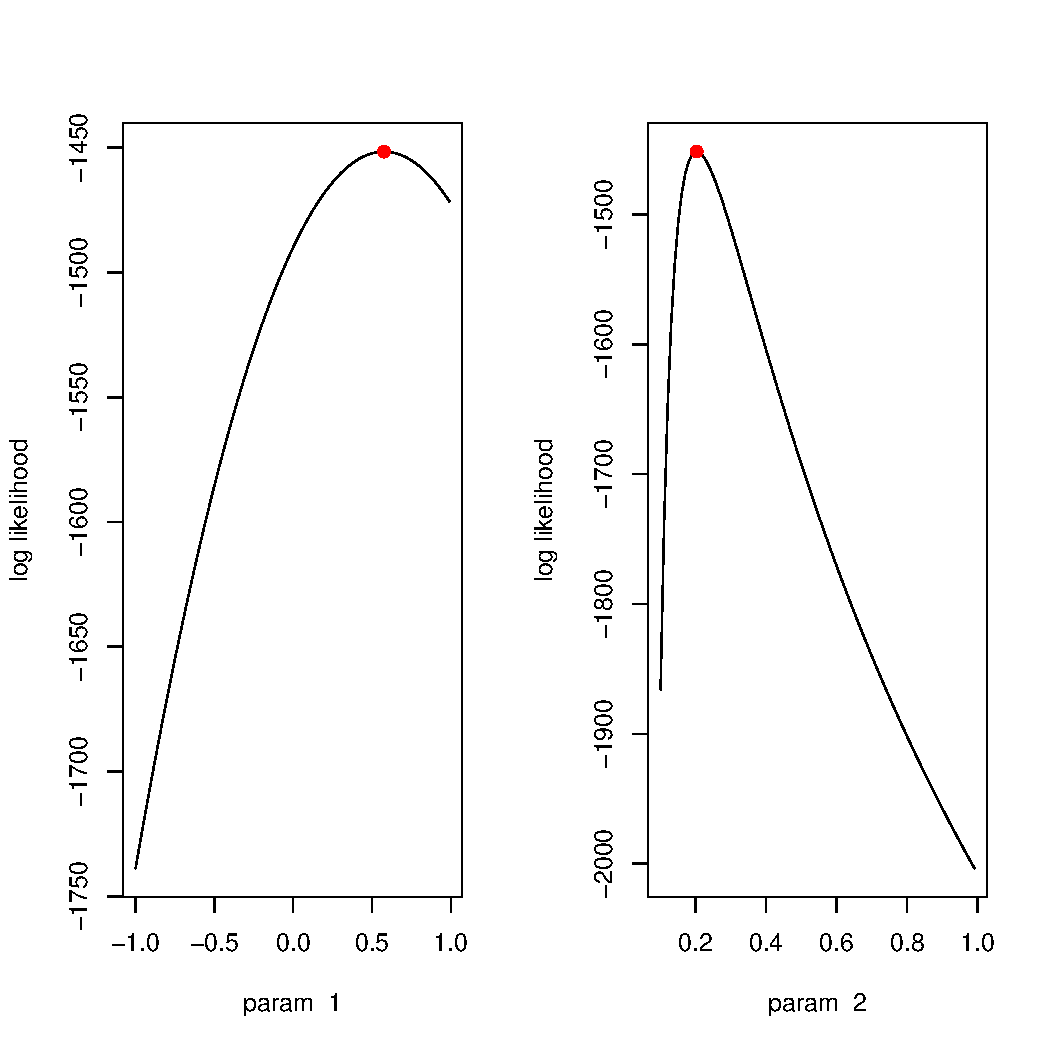
\includegraphics[scale=0.8]{../figures/MLE_GBM.pdf}
\caption{This figure shows the marginal log likelihood function with respect to each parameter of the geometric brownian diffusion model. The mean is represented by Parameter 1 and the volatility by Parameter 2.}
\label{fig:mle_gbm}
\end{figure}

\begin{table}[h!]
\begin{tabular}{c|cc}
\hline
 & $\mu$ &   $\sigma$ \\
\hline
Actual & $0.5$ & $0.2$ \\
Estimated & $0.525$ & $0.204$  \\
Est. Std. Error & $6.415 \times 10^{-2}$ & $5.975\times 10^{-3}$ \\
Est. Huber Sandwich Error & $6.420 \times 10^{-2}$ & $6.624\times 10^{-3}$ \\
Error in Est. Std. Error & $5.169 \times 10^{-13}$ & $9.339\times 10^{-12}$ \\
Error in Est. Huber Sandwich Error & $4.214\times 10^{-13}$ & $7.931\times 10^{-12}$ \\
\hline
\end{tabular}
\caption{This table lists the correct parameters, the estimates and the standard error estimates using 500 simulated stock prices.}
\label{tab:gbm}
\end{table}


\begin{table}[h!]
\begin{tabular}{c|c}
\hline
Actual maximum log likelihood & $1326.4464$\\
Est. maximum log likelihood &  $1326.204$\\
L2 Norm of Score Error & $1.659 \times 10^{7}$\\
L2 Norm of Hessian Error & $1.448 \times 10^{7}$\\
L2 Norm of Information matrix &  $1.962 \times 10^{6}$\\
\hline
\end{tabular}
\caption{This table lists the numerical error in a selection of estimated values.}
\label{tab:gbm2}
\end{table}


\subsection{Heston Model}
All results are presented for the case when there are $n=50$ simulated weekly observations using an Euler scheme with 10 intermediate time steps between each observations, for a total of 500 time steps. 
The approximate marginal log likelihood function for the state variable $G_t$ with respect to $\rho$ (parameter 1), $\kappa$ (parameter 2), $\theta$ (parameter 3) and $\sigma$ (parameter 4) are given by Figure \ref{fig:mle_heston}. In each case, the red point show the maximum likelihood estimate.  Table \ref{tab:heston} lists the various error estimates.

\begin{figure}[h!]
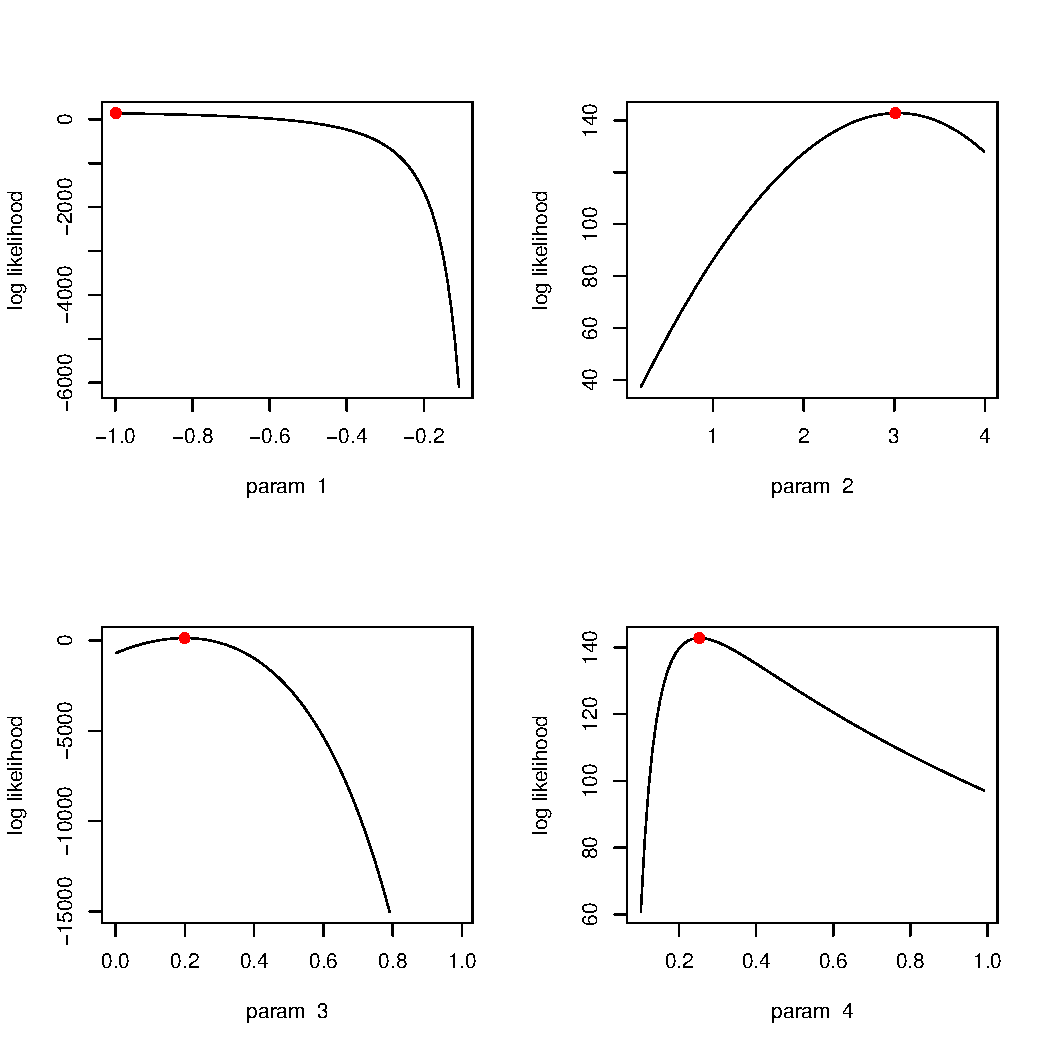
\includegraphics[scale=0.8]{../figures/MLE_Heston.pdf}
\caption{This figure shows the marginal log likelihood function with respect to each parameter of the Heston model applied to the simulated underlying and prices. Parameters 1-4 represents $\rho$, $\kappa$, $\theta$ and $\sigma$.}
\label{fig:mle_heston}
\end{figure}

\begin{table}[h!]
\begin{tabular}{c|cccc}
\hline
 & $\rho$ &   $\kappa$ &  $\theta$ &  $\sigma$\\
\hline
Actual & $-0.8$ & $3.0$ & $0.2$ & $0.25$ \\
Estimated & $-0.81$ & $3.4$ & $0.201$ & $0.2476$ \\
Std. Error & $6.702 \times 10^{-3}$ & $1.092 $ & $1.496\times 10^{-3}$ & $4.687\times 10^{-2}$\\
Huber Sandwich Error & $4.903 \times 10^{-4}$ & $9.311 \times 10^{-1}$ & $1.117\times 10^{-2}$ & $3.356\times 10^{-2}$\\
\hline
\end{tabular}
\caption{This table lists the correct parameters, the estimates and the lower bounds on the standard error using 50 simulated observations of the stock and the ATM option price.}
\label{tab:heston}
\end{table}
Figures \ref{fig:heston_err_price} and \ref{fig:heston_vol_price} show the absolute error in the calibrated model option prices and volatilities versus the simulated states ${g_t}_{i=1}^n$ at weekly intervals.


\begin{figure}
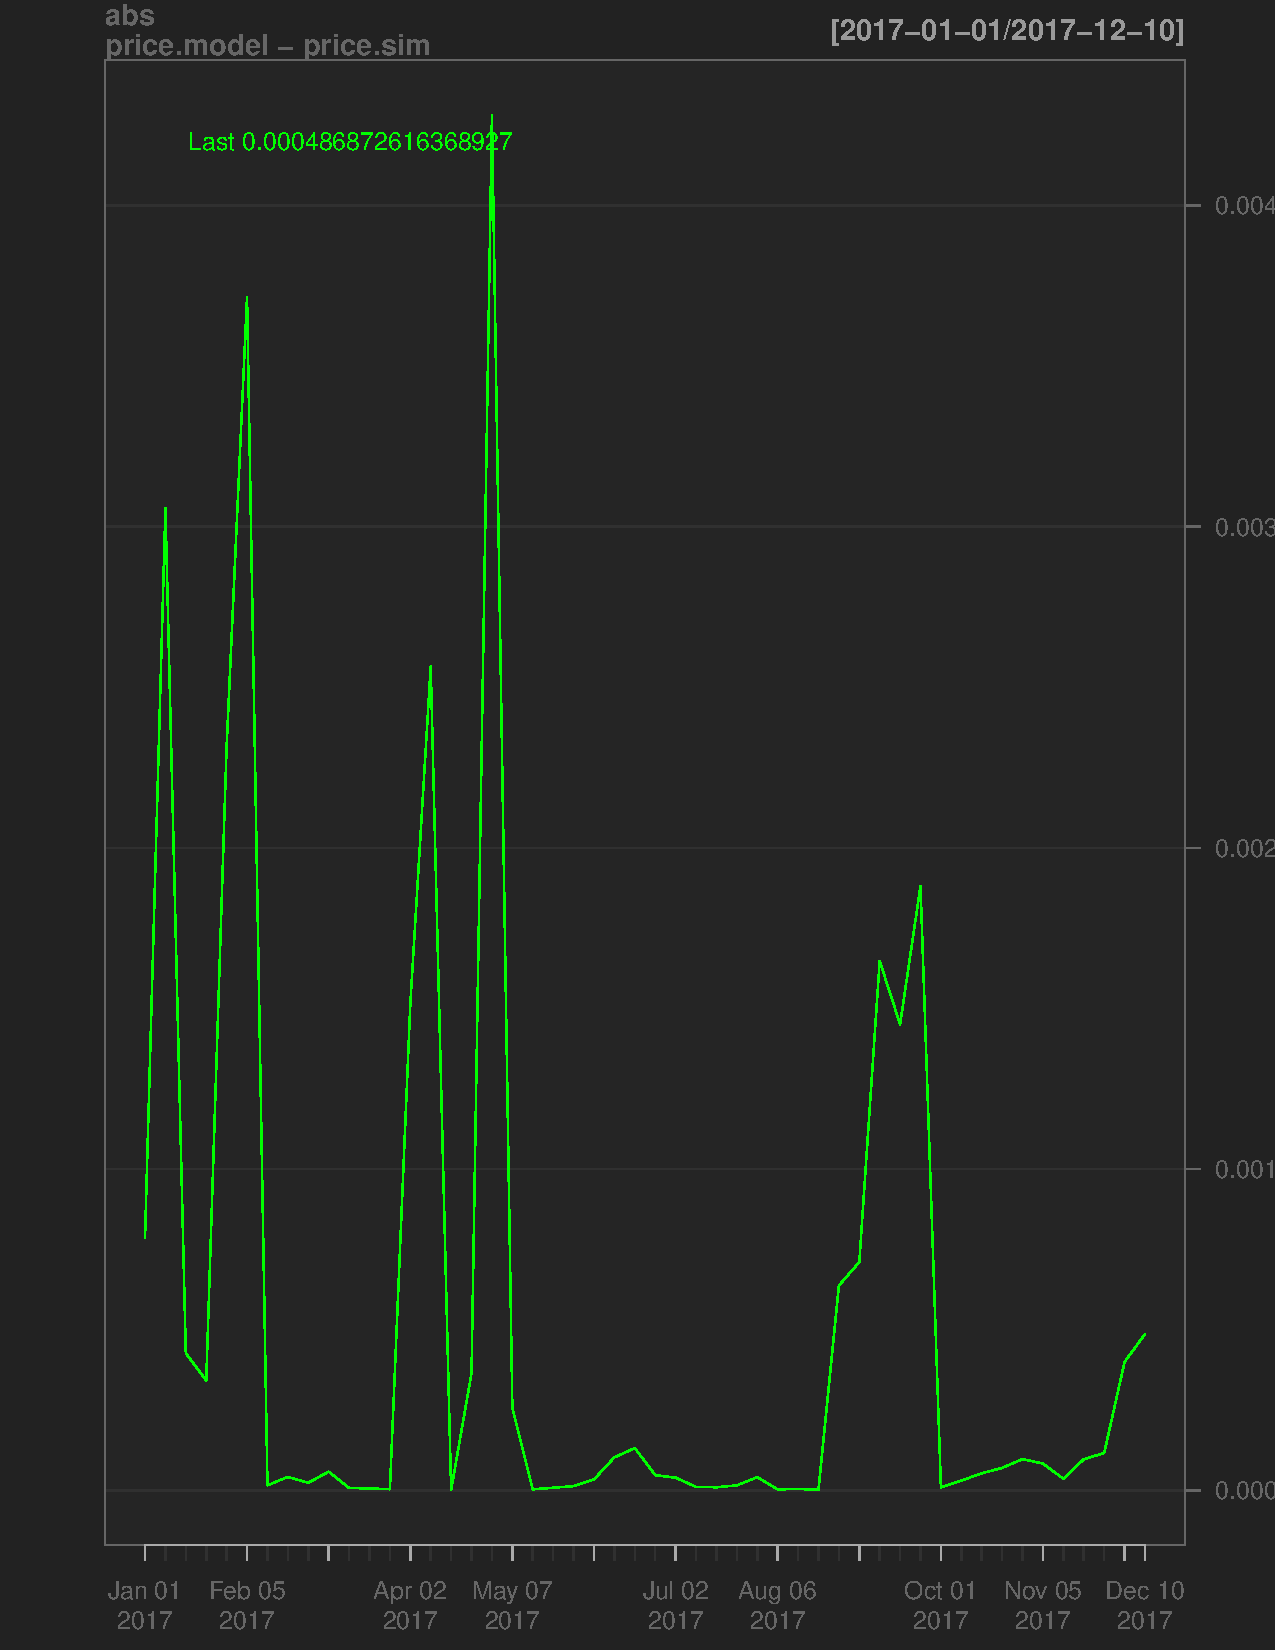
\includegraphics[scale=0.6]{../figures/Heston_err_price.pdf}
\caption{This figure shows the absolute error in the calibrated model prices versus the simulated prices.}
\label{fig:heston_err_price}
\end{figure}

\begin{figure}
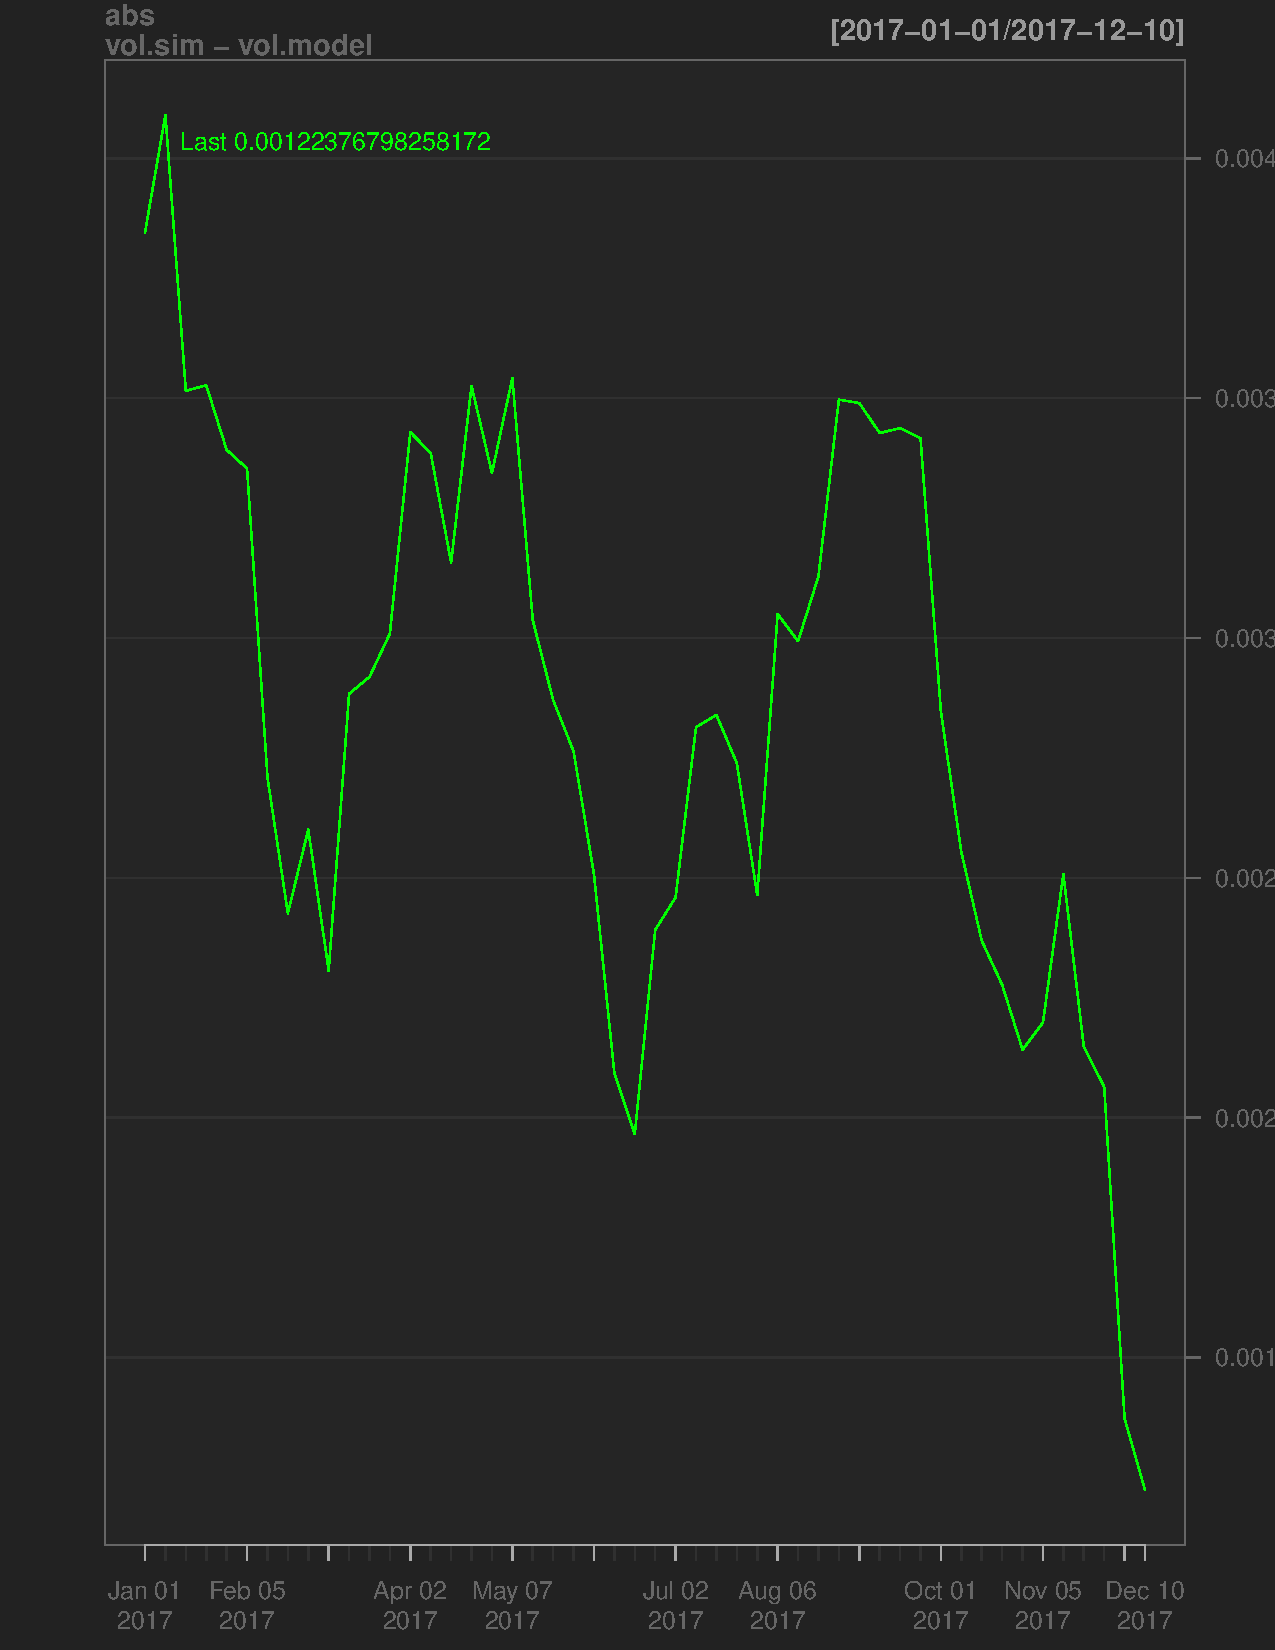
\includegraphics[scale=0.6]{../figures/vol_error.pdf}
\caption{This figure shows the absolute error in the implied volatilities versus the simulated volatilities.}
\label{fig:heston_vol_price}
\end{figure}

\section{Conclusion}
Continuous-time Markov processes are typically defined by stochastic differential equations, describing the evolution of one or more state variables. Maximum likelihood estimation of the model parameters to historical observations is only possible when at least one of the state variables is observable. In these cases, the form of the transition function corresponding to the stochastic differential equations must be known to assess the efficacy of fitting a continuous model to discrete samples.  This paper makes two contributions:  (i) we describe a R package \verb|MLEVD| for calibrating general multi-variate diffusions models using maximum likelihood estimates; and (ii) we present an algorithm for calibrating the Heston model to option prices using maximum likelihood estimation and assess the robustness of the approach using Monte Carlo simulation. In future works we seek to extend this approach to calibrating to historical observations of the implied volatility surface.
\clearpage

\appendix

\section{Overview of Package} \label{sect:MLEMVD}

[To do: Describe the purpose of this package.]

\section{Model Reference}\label{sect:model_examples}
\begin{table}[h!]
\begin{tabular}{|c|c|c|c|}
\hline
Model & $\mu$ & $\sigma$ & constraints\\
\hline
U1 & $x(a+bx)$ & $\sigma x^{3/2}$ & \\
\hline
U2 & $a+bx$ &$dx$& \\
\hline
U3 & $b(a-x)$ & $cx^d$& \\
\hline
U4 & $\kappa(\alpha-x)$ & $\sigma x^{1/2}$& \\
\hline
U5 & $\sum_{i=0}^3 \theta_ix^i$ & $\gamma x^{\rho}$& $\rho\geq 1$\\
\hline
U6 & $a+bx+cx^2+dx^3$ & $f$ & \\
\hline
U7 & $\kappa(\alpha-x)$ & $\sigma$ & \\
\hline
U8 & $\frac{a_{-1}}{x} + a_0 + a_1x+ a_2x^2$ & $\sigma x^p$ & $\rho\geq 1$\\
\hline
U9 & $\frac{a_{-1}}{x} + a_0 + a_1x+ a_2x^2$ & $(b_0 +b_1x+b_2x^{b_3})^{1/2}$ & \\
\hline
U10 & $\frac{a_{-1}}{x} + a_0 + a_1x+ a_2x^2$ & $b_0 +b_1x+b_2x^{b_3}$ & $\rho\geq 1$\\
\hline
U11 & $a+bx$ & $f+dx$ &\\
\hline
U12 & $\frac{\beta}{x}-\alpha x^3$ & $\gamma x^{1/2}$ & \\
\hline
U13 & $\frac{a_{-1}}{x} + a_0 + a_1x+ a_2x^2 +a_3x^3$ & $\sigma x^{\rho}$ & $\rho\geq 1$\\
\hline
\end{tabular}
\caption{The specification of various univariate diffusion models currently supported by the package.}
\end{table}



\begin{table}[h!]
\tiny{
\begin{tabular}{|c|c|c|c|}
\hline
Model & $\mu(x_1,x_2)$ & $\Sigma(x_1,x_2)$ & constraints\\
\hline
B1 & $\left( \begin{array}{c} a+bx_2\\ c+dx_2 \end{array} \right)$ & $\left( \begin{array}{cc} \rho\sqrt(x_2) & 0\\ h & \sqrt{(1-\rho^2)x_2} \end{array} \right)$ & \\
\hline
B2 & $\left( \begin{array}{c} a_0+a_1x_1+a_2x_2\\ b_0+b_1x_1+b_2x_2 \end{array} \right)$ &
$\left( \begin{array}{cc} c_0+c_1x_1+c_2x_2 & 0\\ 0 & d_0+d_1x_1+d_2x_2 \end{array} \right)$ & \\
\hline
B3 & $\left( \begin{array}{c} \mu -x_2/2\\ \alpha + \beta x_2 \end{array} \right)$ &
$\left( \begin{array}{cc} \sqrt{x_2} & 0\\ \sigma\rho x_2^{\gamma} & \sigma \sqrt{1-\rho^2}x^{\gamma}_2 \end{array} \right)$ & \\
\hline
B4 & $\left( \begin{array}{c} a_0+a_1x_2\\ b(a-x_2) + \lambda g x_2^{\beta}\sqrt{a+f(x_2-a)} \end{array} \right)$ &
$\left( \begin{array}{cc}\sqrt{1-\rho^2}\sqrt{a+f(x_2-a)} & \rho\sqrt{a+f(x_2-a)}\\ 0 & g x^{\beta}_2 \end{array} \right)$ & \\
\hline
B5 & $\left( \begin{array}{c} bx_1\\ c-dx_2 \end{array} \right)$ &
$\left( \begin{array}{cc} hx_1\sqrt{x_2} & 0\\ g\rho \sqrt{x_2} & g \sqrt{1-\rho^2}\sqrt{x_2} \end{array} \right)$ & \\
\hline
B6 & $\left( \begin{array}{c} m - x_2/2\\ a-bx_2 \end{array} \right)$ &
$\left( \begin{array}{cc} \sqrt{x_2} & 0\\ \sigma \sqrt{1-\rho^2}\sqrt{x_2} & \sigma \rho\sqrt{x_2} \end{array} \right)$ & $2a> \sigma^2$ \\
\hline
B7 & $\left( \begin{array}{c} 0\\ a_1-a_2x_2 \end{array} \right)$ &
$\left( \begin{array}{cc} \frac{2x_1}{\gamma\sqrt{x_2}} & \frac{2\eta x_1}{\gamma}\\ 2\sqrt{x_2} & 0 \end{array} \right)$ &  \\
\hline
B8 & $\left( \begin{array}{c} a+bx_1\\ cx_2 \end{array} \right)$ &
$\left( \begin{array}{cc} dx_1^{\gamma}e^{x_2} & 0\\ 0 & f \end{array} \right)$ &  \\
B9 & $\left( \begin{array}{c} a+bx_1\\ cx_2 \end{array} \right)$ &
$\left( \begin{array}{cc} dx_1^{\gamma}e^{x_2} & 0\\ 0 & f \end{array} \right)$ &  \\
\hline
B10 &
$\left( \begin{array}{c} b_1(a_1-x_1)\\ b_2(a_2-x_2) \end{array} \right)$ &
$\left( \begin{array}{cc} g_1 & 0\\ 0 & g_2\sqrt{x_2} \end{array} \right)$ &
\\

\hline
B11 &
$\left( \begin{array}{c} k_1 + k_2x_2\\ \kappa(\theta-x_2) \end{array} \right)$ &
$\left( \begin{array}{cc} \sqrt{1-\rho^2}\sqrt{x_2} & \rho\sqrt{x_2}\\ 0 & \sigma x_2 \end{array} \right)$ &
\\

\hline
B12 &
$\left( \begin{array}{c} ax_1\\ -bx_2 \end{array} \right)$ &
$\left( \begin{array}{cc} cx_1e^{x_2} & 0\\ dr & d\sqrt{1-r^2} \end{array} \right)$ &
\\

\hline
B13 &
$\left( \begin{array}{c} b_{11}(a_1-x_1) + b_{12}(a_2-x_2)\\ b_{21}(a_1-x_1) + b_{22}(a_2-x_2) \end{array} \right)$ &
$\left( \begin{array}{cc} \sigma_{11} & \sigma_{12}\\ \sigma_{21} & \sigma_{22} \end{array} \right)$ &
\\

\hline
B14 &
$\left( \begin{array}{c} k_1(x_2-x_1)\\ k_2(\theta-x_2) \end{array} \right)$ &
$\left( \begin{array}{cc} \sigma\sqrt{x_1} & 0\\ 0 & \sigma_2\sqrt{x_2} \end{array} \right)$ &
\\

\hline
B15 &
$\left( \begin{array}{c} a+bx_1\\ fx_1 + dx_2 \end{array} \right)$ &
$\left( \begin{array}{cc} \sqrt{x_1} & 0\\ h & \sqrt{1+gx_1} \end{array} \right)$ &
\\

\hline
B16 &
$\left( \begin{array}{c} a+bx_1+gx_2\\ d + \eta x_1 + fx_2 \end{array} \right)$ &
$\left( \begin{array}{cc} \sqrt{x_1} & 0\\ h & \sqrt{x_2} \end{array} \right)$ &
\\

\hline
B17 &
$\left( \begin{array}{c} a_{00}-(a_1+a_2x_2)/2+(n_0\sqrt{1-g_1^2} + nu_1g_1)(\sqrt{a_1 + a_2x_2}^{b+d}\\ a_{01}+a_{11}x_2+(nu_1g_{11})(\sqrt{a_1+a_2x_2}^{b+d} \end{array} \right)$ &
$\left( \begin{array}{cc} \sqrt{1-g_1^2}\sqrt{a_1+a_2x_2} & g_1\sqrt{a_1+a_2x_2}\\ 0 & g_{11}(\sqrt{a_1+a_2x_2})^b \end{array} \right)$ &
\\

\hline
B18 &
$\left( \begin{array}{c} b_1x_1\\ a_2+b_2x_2 \end{array} \right)$ &
$\left( \begin{array}{cc} g_{11}e^{x_1} & 0\\ g_{22}r & g_{22}\sqrt{1-r^2} \end{array} \right)$ &
\\

\hline
B19 &
$\left( \begin{array}{c} b_1x_1\\ a_2+b_2x_2 \end{array} \right)$ &
$\left( \begin{array}{cc} e^{x_2} & 0\\ g_{22}r & g_{22}\sqrt{1-r^2} \end{array} \right)$ &
\\

\hline
B20 &
$\left( \begin{array}{c} a_1+b_1x_1\\ a_2+b_2x_2 \end{array} \right)$ &
$\left( \begin{array}{cc} \sqrt{x_2} & 0\\ gr\sqrt{x_2} & g\sqrt{1-r^2}\sqrt{x_2} \end{array} \right)$ &
\\

\hline
B21 &
$\left( \begin{array}{c} a_1(b_1-x_1)\\ a_{21}(b_1-x_1)+a_2(b_2-x_2) \end{array} \right)$ &
$\left( \begin{array}{cc} \sqrt{x_1} & 0\\ g_{21}\sqrt{x_1} & g_{22}\sqrt{x_1} \end{array} \right)$ &
\\

\hline
B22 &
$\left( \begin{array}{c} k_1+k_2x_2\\ k(a-x_2) \end{array} \right)$ &
$\left( \begin{array}{cc} \sqrt{1-r^2}\sqrt{x_2} & r\sqrt{x_2}\\ 0 & sx_2^b \end{array} \right)$ &
\\
\hline

\end{tabular}
}
\caption{The specification of various bivariate diffusion models currently supported by the package.}
\end{table}

\clearpage

\bibliographystyle{abbrv}
\bibliography{PackageDescription}

\end{document}



